\section{Spring Problems II}

\boxit{Free Vibrations With Damping}

\noindent
In this section we consider the motion of an object in a spring--mass
system with damping. We start with unforced motion, so the equation of
motion is
\begin{equation}\label{eq:6.2.1}
my''+cy'+ky=0.
\end{equation}
Now suppose   the object is displaced from equilibrium and given an
initial velocity. Intuition suggests that if the damping force is
sufficiently weak the resulting motion will be oscillatory, as in the
undamped case considered in the previous section, while if it's
sufficiently strong the object may just move slowly toward the
equilibrium
position without ever reaching it. We'll now confirm these intuitive
ideas mathematically. The characteristic equation of \eqref{eq:6.2.1} is
$$
mr^2+cr+k=0.
$$
The roots of this equation are
\begin{equation}\label{eq:6.2.2}
r_1={-c-\sqrt{c^2-4mk}\over2m}\mbox{\quad and \quad} r_2=
{-c+\sqrt{c^2-4mk}\over2m}.
\end{equation}
In Section~5.2 we saw that the form of the
solution of  \eqref{eq:6.2.1} depends upon whether $c^2-4mk$ is positive,
negative, or zero. We'll now consider these three cases.

\boxit{Underdamped Motion}

\noindent
We say the motion is {\color{blue}\it underdamped\/} if $c<\sqrt{4mk}$. In this
case $r_1$ and $r_2$ in \eqref{eq:6.2.2} are complex conjugates, which we
write as
$$
r_1=-{c\over2m}-i\omega_1\mbox{\quad and \quad}
r_2=-{c\over2m}+i\omega_1,
$$
where
$$
\omega_1={\sqrt{4mk-c^2}\over2m}.
$$
The general solution of  \eqref{eq:6.2.1} in this case is
$$
y=e^{-ct/2m}(c_1\cos\omega_1 t+c_2\sin\omega_1 t).
$$
By the method used in Section~6.1 to derive the
amplitude--phase form of the displacement of an object in simple
harmonic motion, we can rewrite this equation as
\begin{equation}\label{eq:6.2.3}
y=Re^{-ct/2m}\cos(\omega_1 t-\phi),
\end{equation}
 where
$$
R=\sqrt{c_1^2+c_2^2},\quad R\cos\phi=c_1,\mbox{\quad and \quad} R\sin\phi=c_2.
$$
The factor $Re^{-ct/2m}$ in \eqref{eq:6.2.3} is called the {\color{blue}\it
time--varying amplitude\/} of the motion, the quantity $\omega_1$ is
called the {\color{blue}\it frequency\/}, and $T=2\pi/\omega_1$ (which is the
period of the cosine function in \eqref{eq:6.2.3} is called the {\color{blue}\it
quasi--period\/}. A typical graph of \eqref{eq:6.2.3} is shown in
Figure~\ref{figure:6.2.1}. As illustrated in that figure, the graph of $y$
oscillates between the dashed exponential curves $y=\pm Re^{-ct/2m}$.

  \begin{figure}[tbp]
  \centering
  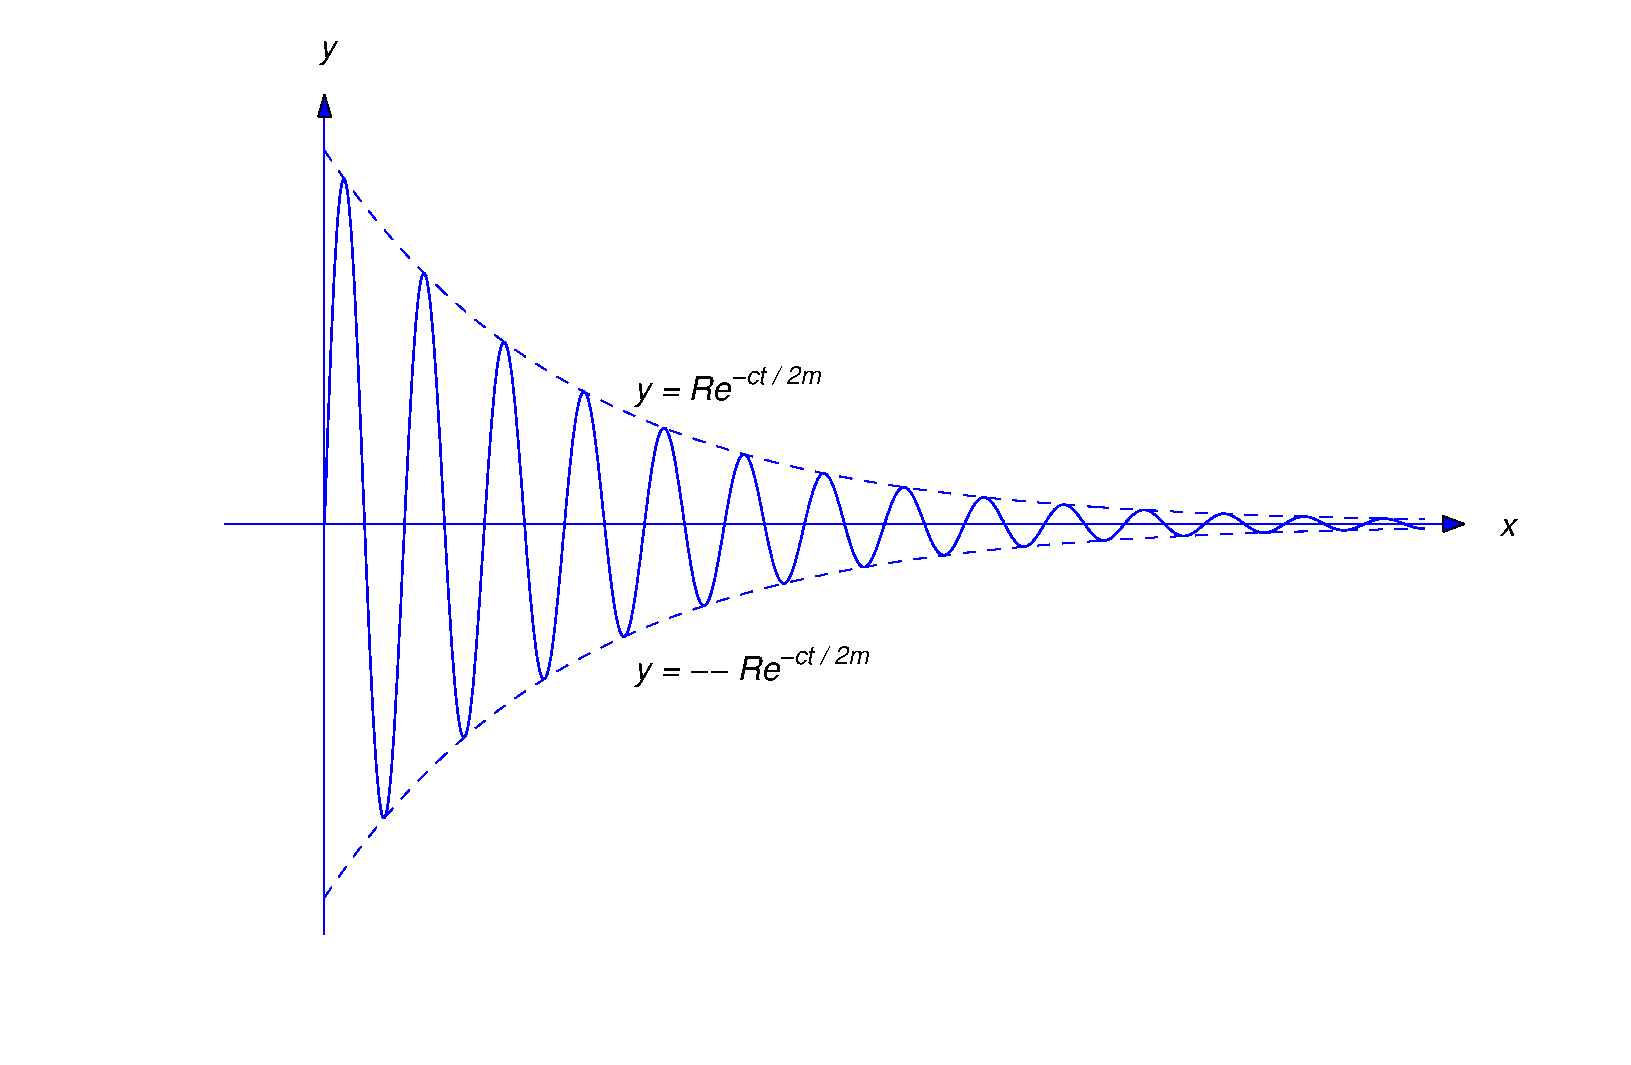
\includegraphics[bb=-78 148 689 643,width=5.67in,height=3.66in,keepaspectratio]{fig060201}
\color{blue}
\caption{ Underdamped motion}
  \label{figure:6.2.1}
\end{figure}

\newpage
\boxit{Overdamped Motion}

\noindent
We say the motion is {\color{blue}\it overdamped\/} if $c>\sqrt{4mk}$. In this
case the zeros $r_1$ and $r_2$ of the characteristic polynomial are
real, with $r_1<r_2<0$ (see \eqref{eq:6.2.2}), and the general solution of
\eqref{eq:6.2.1} is
$$
y=c_1e^{r_1t}+c_2e^{r_2t}.
$$
Again $\lim_{t\to\infty}y(t)=0$ as in the
underdamped case, but the motion isn't  oscillatory, since $y$ can't
equal zero for more than one value of $t$ unless $c_1=c_2=0$.
(Exercise~\ref{exer:6.2.23}.)

\boxit{Critically Damped Motion}

\noindent
We say the motion is {\color{blue}\it critically damped\/} if $c=\sqrt{4mk}$. In
this case $r_1=r_2=-c/2m$ and the general solution of \eqref{eq:6.2.1} is
$$
y=e^{-ct/2m}(c_1+c_2t).
$$

Again $\lim_{t\to\infty}y(t)=0$ and the motion is nonoscillatory,
since $y$ can't equal zero for more than one value of $t$ unless
$c_1=c_2=0$. (Exercise~\ref{exer:6.2.22}).

\begin{example}\label{example:6.2.1}\rm
Suppose a 64 lb weight stretches a spring 6 inches in equilibrium
and a dashpot provides a damping force of $c$ lb for each ft/sec of
velocity.
\begin{alist}
\item % (a)
 Write the equation of motion of the object and determine the value of
$c$ for which the motion is critically damped.
\item % (b)
 Find the displacement $y$ for $t>0$ if the motion is critically damped
and the initial conditions are $y(0)=1$ and $y'(0)=20$.
\item % (c)
 Find the displacement $y$ for $t>0$ if the motion is critically damped
and the initial conditions are $y(0)=1$ and $y'(0)=-20$.
\end{alist}
\end{example}

\solutionpart{a}  Here $m=2$ slugs and $k=64/.5=128$
lb/ft. Therefore the equation of motion  \eqref{eq:6.2.1} is
\begin{equation}\label{eq:6.2.4}
2y''+cy'+128y=0.
\end{equation}
The characteristic equation  is
$$
2r^2+cr+128=0,
$$
which has  roots
$$
r={-c\pm\sqrt{c^2-8\cdot128}\over4}.
$$
Therefore the damping is critical if
$$
c=\sqrt{8\cdot128}=32\mbox{ lb--sec/ft}.
$$

\solutionpart{b}
 Setting $c=32$ in  \eqref{eq:6.2.4} and cancelling the common factor $2$
yields
$$
y''+16y+64y=0.
$$
The characteristic equation  is
$$
r^2+16r+64y=(r+8)^2=0.
$$
Hence, the general solution is
\begin{equation}\label{eq:6.2.5}
y=e^{-8t}(c_1+c_2t).
\end{equation}
 Differentiating this yields
\begin{equation}\label{eq:6.2.6}
y'=-8y+c_2e^{-8t}.
\end{equation}
Imposing the initial conditions $y(0)=1$ and $y'(0)=20$ in the last
two equations shows that $1=c_1$ and $20=-8+c_2$. Hence, the solution
of the initial value problem is
$$
y=e^{-8t}(1+28t).
$$
Therefore the object approaches equilibrium from above as
$t\to\infty$. There's no oscillation.
\solutionpart{c}
Imposing the initial conditions $y(0)=1$ and $y'(0)=-20$ in
\eqref{eq:6.2.5} and \eqref{eq:6.2.6} yields $1=c_1$ and $-20=-8+c_2$. Hence,
the solution of this initial value problem is
$$
y=e^{-8t}(1-12t).
$$
Therefore the object moves downward through equilibrium just once,
and then approaches equilibrium from below as $t\to\infty$. Again,
there's no oscillation. The solutions of these two initial value
problems are graphed in Figure~\ref{figure:6.2.2}.

\begin{figure}[tbp]
  \centering
  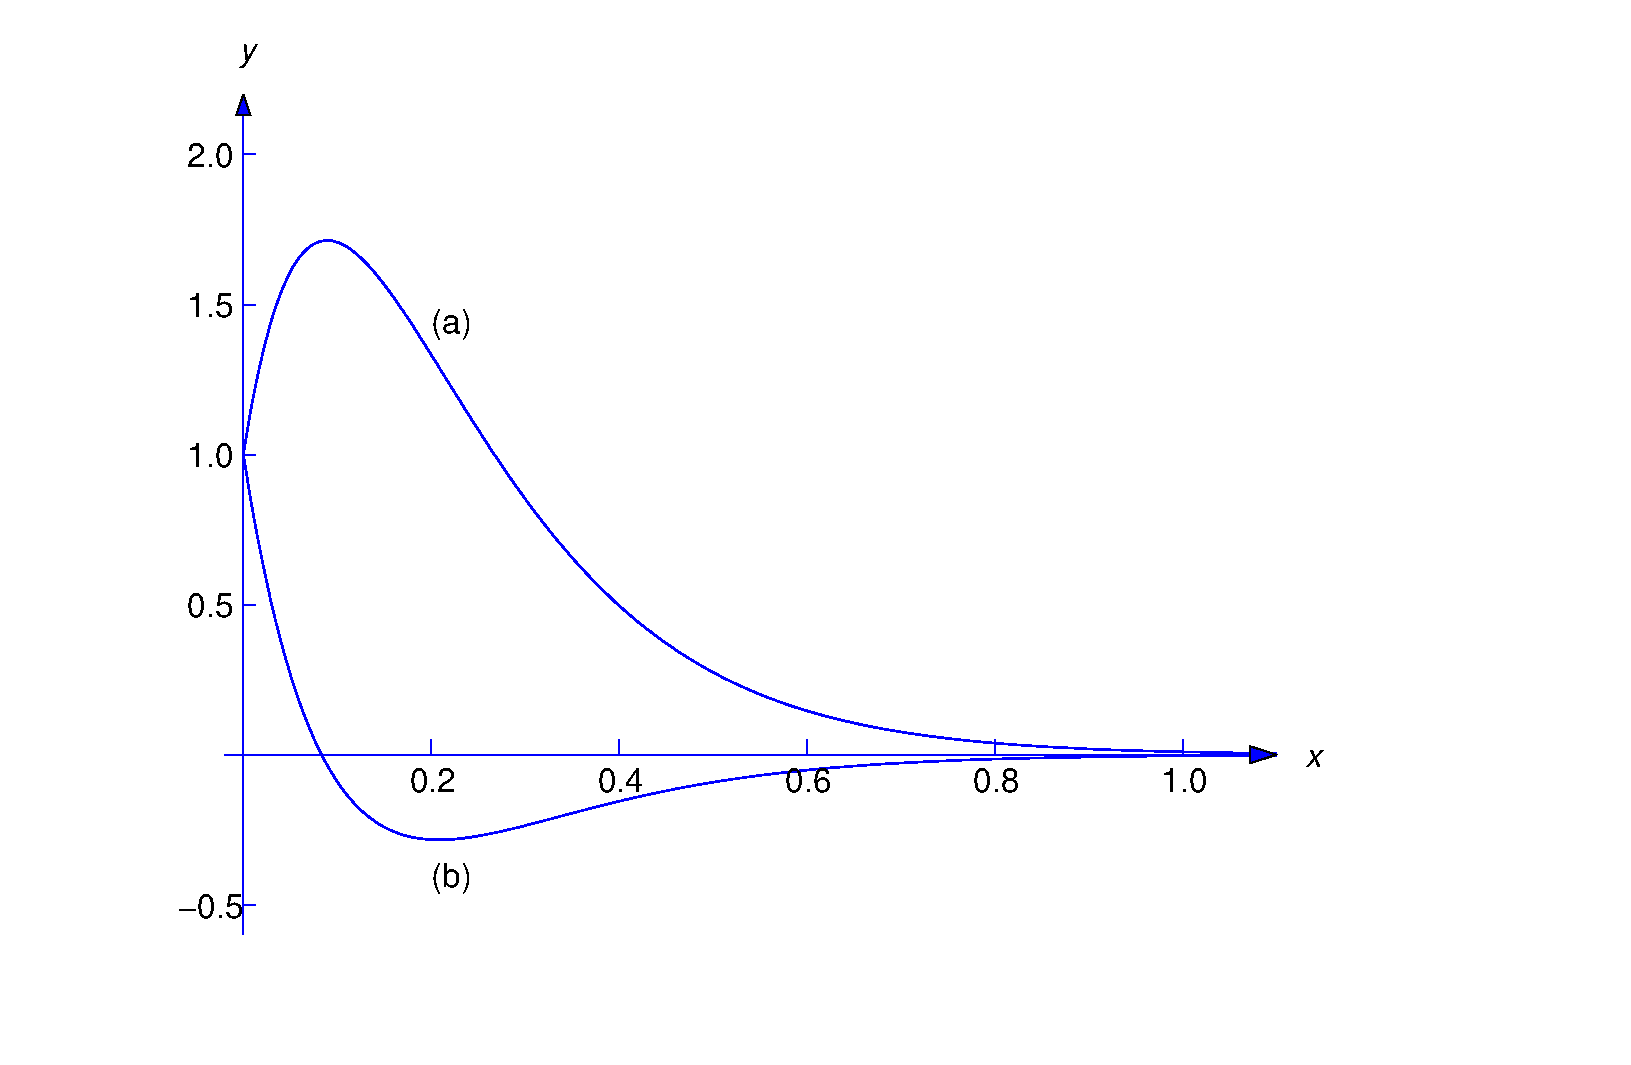
\includegraphics[bb=-78 148 689 643,width=5.67in,height=3.66in,keepaspectratio]{fig060202}
\color{blue}
\caption{ {\bf(a)}\, $y=e^{-8t}(1+28t)$\quad
{\bf (b)}\, $y=e^{-8t}(1-12t)$}
  \label{figure:6.2.2}
\end{figure}

\begin{example}
\label{example:6.2.2}\rm
Find the displacement of the object in Example~\ref{example:6.2.1} if the
damping constant is $c=4$ lb--sec/ft and the initial conditions are
$y(0)=1.5$ ft and $y'(0)=-3$ ft/sec.
\end{example}

\solution
With $c=4$, the equation of motion \eqref{eq:6.2.4} becomes
\begin{equation}\label{eq:6.2.7}
y''+2y'+64y=0
\end{equation}
after cancelling the common factor 2. The characteristic equation
$$
r^2+2r+64=0
$$
has complex conjugate roots
$$
r={-2\pm\sqrt{4-4\cdot64}\over2}=-1\pm3\sqrt7i.
$$
Therefore the motion is underdamped and the
general solution of  \eqref{eq:6.2.7} is
$$
y=e^{-t}(c_1\cos3\sqrt7t+c_2\sin3\sqrt7t).
$$
Differentiating this yields
$$
y'=-y+3\sqrt7e^{-t}(-c_1\sin3\sqrt7t+c_2\cos3\sqrt7t).
$$
Imposing the initial conditions $y(0)=1.5$ and $y'(0)=-3$ in the last
two equations yields $1.5=c_1$ and $-3=-1.5+3\sqrt7c_2$. Hence, the
solution of the initial value problem is
\begin{equation}\label{eq:6.2.8}
y=e^{-t}\bigg({3\over2}\cos3\sqrt7t-{1\over2\sqrt7}
\sin3\sqrt7t\bigg).
\end{equation}
 The amplitude of the function in parentheses is
$$
 R=\sqrt{\bigg({3\over2}\bigg)^2+\bigg({1\over2\sqrt7}\bigg)^2}
=\sqrt{{9\over4}+{1\over4\cdot7}}
=\sqrt{64\over4\cdot7}={4\over\sqrt7}.
$$
Therefore we can rewrite  \eqref{eq:6.2.8} as
$$
y={4\over\sqrt7}e^{-t}\cos(3\sqrt7t-\phi),
$$
 where
$$
\cos\phi={3\over2R}={3\sqrt7\over8}\mbox{\quad and \quad}\sin\phi=-{1\over2\sqrt7R}=
-{1\over8}.
$$
Therefore $\phi\cong-.125$  radians.

\begin{example}\label{example:6.2.3}\rm
Let the damping constant in Example 1 be $c=40$ lb--sec/ft. Find the
displacement $y$ for $t>0$ if $y(0)=1$ and $y'(0)=1$.
\end{example}

\solution
With $c=40$, the equation of motion \eqref{eq:6.2.4} reduces to
\begin{equation}\label{eq:6.2.9}
y''+20y'+64y=0
\end{equation}
 after cancelling the  common factor 2.
The characteristic equation
$$
r^2+20r+64=(r+16)(r+4)=0
$$
 has the roots $r_1=-4$ and $r_2=-16$.  Therefore the general
solution of  \eqref{eq:6.2.9} is
\begin{equation}\label{eq:6.2.10}
y=c_1e^{-4t}+c_2e^{-16t}.
\end{equation}
 Differentiating this yields
$$
y'=-4e^{-4t}-16c_2e^{-16t}.
$$
The last two equations and the initial conditions $y(0)=1$ and $y'(0)=1$
imply that
$$
\begin{array}{rlrl}
c_1&+&c_2&=1\\
-4c_1&-&16c_2&=1.
\end{array}
$$
 The solution of this system is $c_1=17/12$, $c_2=-5/12$.
Substituting these into  \eqref{eq:6.2.10} yields
$$
y={17\over12}e^{-4t}-{5\over12}e^{-16t}
$$
as the solution of the given initial value problem
(Figure~\ref{figure:6.2.3}).

\begin{figure}[tbp]
  \centering
  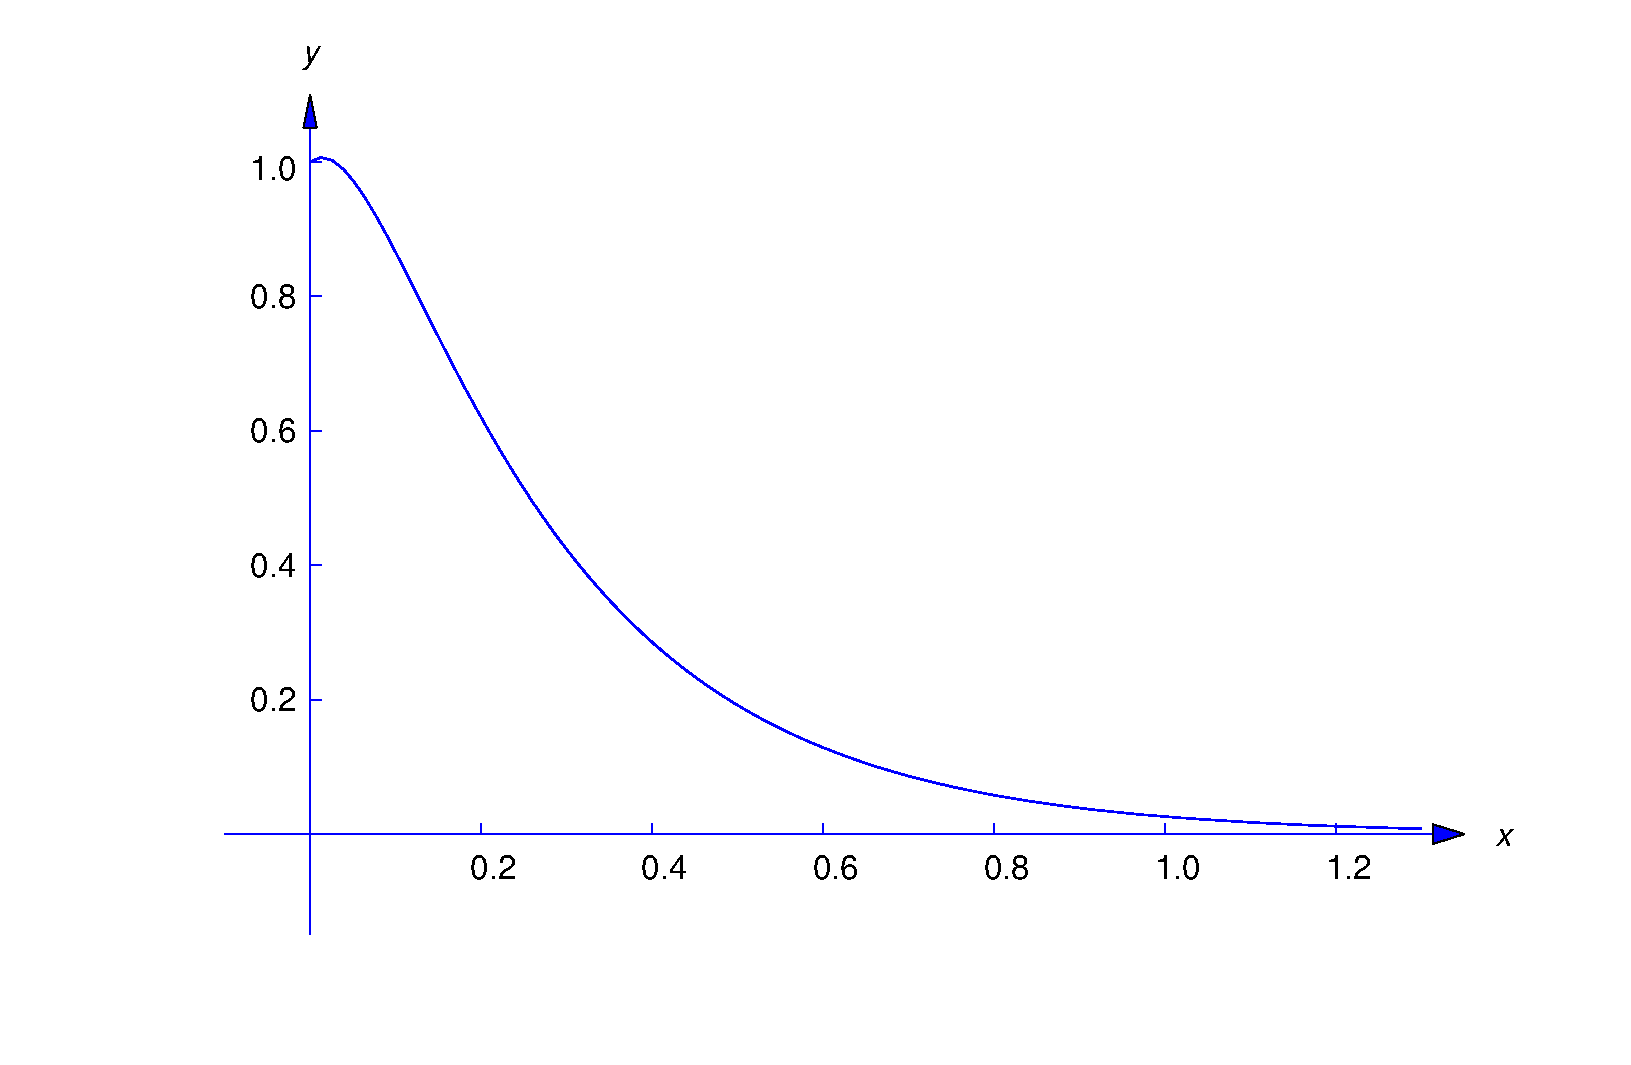
\includegraphics[bb=-78 148 689 643,width=5.67in,height=3.66in,keepaspectratio]{fig060203}
\color{blue}
\caption{$y=\dst{{17\over12}e^{-4t}-{5\over12}e^{-16t}}$}
  \label{figure:6.2.3}
\end{figure}

\boxit{Forced Vibrations With Damping}

\noindent
Now we consider the motion of an object in a spring-mass system with
damping, under the influence of a periodic forcing function
$F(t)=F_0\cos\omega t$, so that the equation of motion is
\begin{equation}\label{eq:6.2.11}
my''+cy'+ky=F_0\cos\omega t.
\end{equation}
In Section~6.1 we considered this equation with $c=0$ and
found that the resulting displacement $y$ assumed arbitrarily large
values in the case of resonance   (that is, when
$\omega=\omega_0=\sqrt{k/m}$). Here we'll see that in the presence
of damping the displacement remains bounded for all $t$, and the
initial conditions have little effect on the motion as $t\to\infty$.
In fact, we'll see that for large $t$ the displacement is closely
approximated by a function of the form
\begin{equation}\label{eq:6.2.12}
y=R\cos(\omega t-\phi),
\end{equation}
where the amplitude $R$ depends upon $m$, $c$, $k$, $F_0$, and
$\omega$. We're interested in the following question:

\bigbox{{\sc Question:}\it Assuming that $m$, $c$, $k$, and $F_0$ are
held constant, what value of $\omega$ produces the largest amplitude
$R$ in {\rm\eqref{eq:6.2.12}}, and what is this largest amplitude?} To
answer this question, we must solve \eqref{eq:6.2.11} and determine $R$ in
terms of $F_0,\omega_0,\omega$, and $c$. We can obtain a particular
solution of \eqref{eq:6.2.11} by the method of undetermined coefficients.
Since $\cos\omega t$ does not satisfy the complementary equation
$$
my''+cy'+ky=0,
$$
we can obtain a particular solution of \eqref{eq:6.2.11} in the form
\begin{equation}\label{eq:6.2.13}
y_p=A\cos\omega t+B\sin\omega t.
\end{equation}
Differentiating this yields
$$
y_p'=\quad\omega (-A\sin\omega t+B\cos\omega t)
$$
and
$$
y_p''=-\omega^2(A\cos\omega t+B\sin\omega t).
$$
 From the last three equations,
$$
my''_p+cy'_p+ky_p=(-m\omega^2A+c\omega B+kA)\cos\omega t+
(-m\omega^2 B-c\omega A+kB)\sin\omega t,
$$
so $y_p$ satisfies  \eqref{eq:6.2.11}  if
$$
\begin{array}{lll}
(k-m\omega^2) A+\quad c\omega B &=&F_0\\
-c\omega A\quad+(k-m\omega^2)B&=&0.
\end{array}
$$

 Solving  for $A$ and $B$
and substituting the results into  \eqref{eq:6.2.13} yields
$$
y_p={F_0\over(k-m\omega^2)^2+c^2\omega^2}
\left[(k-m\omega^2)\cos\omega t+c\omega\sin\omega t\right],
$$
which can be written in amplitude--phase form  as
\begin{equation}\label{eq:6.2.14} %\springsteady
y_p={F_0\over\sqrt{(k-m\omega^2)^2+c^2\omega^2}}
\cos(\omega t-\phi),
\end{equation}
where
\begin{equation}\label{eq:6.2.15}
\cos\phi={k-m\omega^2\over\sqrt
{(k-m\omega^2)^2+c^2\omega^2}}\mbox{\quad and \quad}
\sin\phi={c\omega\over\sqrt{(k-m\omega^2)^2+c^2\omega^2}}.
\end{equation}

  To compare this with the undamped forced vibration
that we considered in Section~6.1 it's useful to write
\begin{equation}\label{eq:6.2.16}
k-m\omega^2=m\bigg({k\over m}-\omega^2\bigg)=
m(\omega_0^2-\omega^2),
\end{equation}
 where $\omega_0=\sqrt{k/m}$ is the natural
angular frequency of the undamped simple harmonic motion of an
object with mass $m$ on a spring with constant $k$.
Substituting  \eqref{eq:6.2.16} into  \eqref{eq:6.2.14} yields
\begin{equation}\label{eq:6.2.17}
y_p={F_0\over\sqrt{m^2(\omega^2_0-\omega^2)^2+
c^2\omega^2}}\cos(\omega t-\phi).
\end{equation}

The solution of an initial value problem
$$
my''+cy'+ky=F_0\cos\omega t, \quad  y(0)=y_0,\quad y'(0)=v_0,
$$
is of the form $y=y_c+y_p$,
where  $y_c$ has one of the three forms
\begin{eqnarray*}
y_c&=&e^{-ct/2m}(c_1\cos\omega_1t+c_2\sin\omega_1t),\\
 y_c&=&e^{-ct/2m}(c_1+c_2t),\\
y_c&=&c_1e^{r_1t}+c_2e^{r_2t}\,(r_1,r_2<0).
\end{eqnarray*}
In all three cases $\lim_{t\to\infty} y_c(t)=0$ for any choice of
$c_1$ and $c_2$. For this reason we say that $y_c$ is the {\color{blue}\it
transient component} of the solution $y$. The behavior of $y$ for
large $t$ is determined by $y_p$, which we call the {\color{blue}\it steady state
component} of $y$. Thus, for large $t$ the motion is like simple
harmonic motion at the frequency of the external force.

The amplitude of $y_p$ in \eqref{eq:6.2.17} is
\begin{equation}\label{eq:6.2.18}
R={F_0\over\sqrt{m^2(\omega^2_0-\omega^2)^2+c^2\omega^2}},
\end{equation}
which is finite for all $\omega$; that is, the presence of damping
precludes the phenomenon of resonance that we encountered in studying
undamped vibrations under a periodic forcing function. We'll now
find the value $\omega_{\max}$ of $\omega$ for which $R$ is maximized.
This is the value of $\omega$ for which the function
$$
\rho (\omega)=m^2(\omega^2_0-\omega^2)^2+c^2\omega^2
$$
in the denominator of  \eqref{eq:6.2.18} attains its minimum value.  By
rewriting this as
\begin{equation}\label{eq:6.2.19}
\rho (\omega)=m^2(\omega^4_0+\omega^4)+
 (c^2-2m^2\omega^2_0)\omega^2,
\end{equation}
 you can see that $\rho$ is a strictly
increasing function of $\omega^2$ if
$$
c\ge\sqrt{2m^2\omega^2_0}=\sqrt{2mk}.
$$
(Recall that $\omega^2_0=k/m$). Therefore $\omega_{\max}=0$ if this
inequality holds. From \eqref{eq:6.2.15}, you can see that $\phi=0$ if
$\omega=0$. In this case, \eqref{eq:6.2.14} reduces to
$$
y_p={F_0\over\sqrt{m^2\omega^4_0}}={F_0\over k},
$$
which is consistent with Hooke's law: if the mass is subjected to a
constant force $F_0$,  its displacement should approach a constant
$y_p$ such that $ky_p=F_0$. Now suppose   $c<\sqrt{2mk}$. Then,
from \eqref{eq:6.2.19},
$$
\rho'(\omega)=2\omega(2m^2\omega^2+c^2-2m^2\omega^2_0),
$$
and $\omega_{\max}$ is the value of $\omega$ for which the
expression in parentheses equals zero; that is,
$$
\omega_{\max}=\sqrt{\omega^2_0-{c^2\over2m^2}}
=\sqrt{{k\over m}\left(1-{c^2\over2km}\right)}.
$$
(To see that $\rho(\omega_{\max})$ is the minimum value of
$\rho(\omega)$, note that $\rho'(\omega)<0$ if $\omega
<\omega_{\max}$ and $\rho'(\omega)>0$ if $\omega>\omega_{\max}$.)
Substituting $\omega=\omega_{\max}$ in \eqref{eq:6.2.18} and simplifying
shows that the maximum amplitude $R_{\max}$ is
$$
R_{\max}={2mF_0\over c\sqrt{4mk-c^2}} \mbox{\quad if \quad} c<
\sqrt{2mk}.
$$
We summarize our results  as follows.

\begin{theorem}\color{blue} \label{thmtype:6.2.1}
 Suppose we consider the amplitude $R$ of the steady state
component of the solution of
$$
my''+cy'+ky=F_0\cos\omega t
$$
as a function of $\omega$.
\newline\indent{\rm(a)} If $c\ge\sqrt{2mk}$,  the maximum amplitude is
 $R_{\max}=F_0/k$ and it's attained when $\omega=
\omega_{\max}=0$.
\newline\indent
{\rm(b)} If $c<\sqrt{2mk}$, the maximum amplitude is
\begin{equation}\label{eq:6.2.20}
R_{\max}={2m F_0\over c\sqrt{4mk-c^2}},
\end{equation}
and it's attained when
\begin{equation}\label{eq:6.2.21}
\omega=\omega_{\max}=\sqrt{{k\over m}\left(1-{c^2\over
2km}\right)}.
\end{equation}
\end{theorem}
Note that $R_{\max}$ and $\omega_{\max}$ are continuous functions
of $c$, for $c\ge0$, since  \eqref{eq:6.2.20} and  \eqref{eq:6.2.21} reduce
to $R_{\max}=F_0/k$ and $\omega_{\max}=0$ if $c=\sqrt{2km}$.

\newpage
\exercises
\begin{exerciselist}

\item\label{exer:6.2.1}
A 64 lb object stretches a spring 4 ft in equilibrium. It is attached
to a dashpot with damping constant $c=8$ lb-sec/ft. The object is
initially displaced 18 inches above equilibrium and given a downward
velocity of 4 ft/sec. Find its displacement and time--varying
amplitude for $t>0$.

\item\label{exer:6.2.2} \CGex
A 16 lb weight is attached to a spring with natural length 5 ft. With
the weight attached, the spring measures 8.2 ft. The weight is
initially displaced 3 ft below equilibrium and given an upward
velocity of 2 ft/sec. Find and graph its displacement
 for $t>0$ if the medium resists the motion with a force of
one lb for each ft/sec of velocity. Also, find its time--varying amplitude.

\item\label{exer:6.2.3} \CGex
An 8 lb weight stretches a spring 1.5 inches. It is attached to a
dashpot with damping constant $c$=8 lb-sec/ft. The weight is
initially displaced 3 inches above equilibrium and given an upward
velocity of 6 ft/sec. Find and graph its displacement for $t>0$.

\item\label{exer:6.2.4}
A 96 lb weight stretches a spring 3.2 ft in equilibrium. It is
attached to a dashpot with damping constant $c$=18 lb-sec/ft. The
weight is initially displaced 15 inches below equilibrium and given a
downward velocity of 12 ft/sec. Find its displacement for $t>0$.

\item\label{exer:6.2.5}
  A 16 lb weight  stretches a spring 6 inches in equilibrium.
It is attached to a damping mechanism with constant $c$.  Find all values
of $c$ such that the free vibration of the weight has infinitely many
oscillations.

\item\label{exer:6.2.6}
An 8 lb weight stretches a spring .32 ft. The weight is initially
displaced 6 inches above equilibrium and given an upward velocity of 4
ft/sec. Find its displacement for $t>0$ if the medium exerts a
damping force of 1.5 lb for each ft/sec of velocity.
\item\label{exer:6.2.7}
A 32 lb weight stretches a spring 2 ft in equilibrium. It is attached
to a dashpot with constant $c=8$ lb-sec/ft. The weight is initially
displaced 8 inches below equilibrium and released from rest. Find its
displacement for $t>0$.

\item\label{exer:6.2.8}
  A mass of 20 gm stretches a  spring 5 cm.  The spring
is attached to a dashpot with damping constant 400 dyne sec/cm.  Determine
the displacement for $t>0$ if the mass is  initially displaced
 9 cm  above equilibrium  and released from rest.

\item\label{exer:6.2.9}
A 64 lb weight is suspended from a spring with constant $k=25$ lb/ft.
It is initially displaced 18 inches above equilibrium and released
from rest. Find its displacement for $t>0$ if the medium resists the
motion with 6 lb of force for each ft/sec of velocity.

\item\label{exer:6.2.10}
A 32 lb weight stretches a spring 1 ft in equilibrium. The weight is
initially displaced 6 inches above equilibrium and given a downward
velocity of 3 ft/sec. Find its displacement for $t>0$ if the medium
resists the motion with a force  equal to 3 times the speed
in ft/sec.

\item\label{exer:6.2.11}
An 8 lb weight stretches a spring 2 inches. It is attached to a
dashpot with damping constant $c$=4 lb-sec/ft. The weight is
initially displaced 3 inches above equilibrium and given a downward
velocity of 4 ft/sec. Find its displacement for $t>0$.

\item\label{exer:6.2.12} \CGex
A 2 lb weight stretches a spring .32 ft. The weight is initially
displaced 4 inches below equilibrium and given an upward velocity of 5
ft/sec. The medium provides damping with constant $c=1/8$ lb-sec/ft.
Find and graph the displacement for $t>0$.

\item\label{exer:6.2.13}
  An 8 lb weight stretches a spring 8 inches in equilibrium.
It is attached to a dashpot with damping constant $c=.5$ lb-sec/ft
and subjected to an external force  $F(t)=4\cos2t$ lb.
Determine the steady state component of the displacement for $t>0$.

\item\label{exer:6.2.14}
A 32 lb weight stretches a spring 1 ft in equilibrium. It is attached
to a dashpot with constant $c=12$ lb-sec/ft. The weight is initially
displaced 8 inches above equilibrium and released from rest. Find its
displacement for $t>0$.

\item\label{exer:6.2.15}
A mass of one kg stretches a spring 49 cm in equilibrium. A dashpot
attached to the spring supplies a damping force of 4 N for each m/sec
of speed. The mass is initially displaced 10 cm above equilibrium and
given a downward velocity of 1 m/sec. Find its displacement for $t>0$.

\item\label{exer:6.2.16}
A mass of 100 grams stretches a spring 98 cm in equilibrium. A dashpot
attached to the spring supplies a damping force of 600 dynes for each
cm/sec of speed. The mass is initially displaced 10 cm above
equilibrium and given a downward velocity of 1 m/sec. Find its
displacement for $t>0$.

\item\label{exer:6.2.17}
A 192 lb weight is suspended from a spring with constant $k=6$ lb/ft
and subjected to an external force $F(t)=8\cos3t$ lb. Find the steady
state component of the displacement for $t>0$ if the medium resists
the motion with a force  equal to 8 times the speed in
ft/sec.

\item\label{exer:6.2.18}
A 2 gm mass is attached to a spring with constant 20 dyne/cm. Find the
steady state component of the displacement if the mass is subjected to
an external force $F(t)=3\cos4t-5\sin4t$ dynes and a dashpot supplies
4 dynes of damping for each cm/sec of velocity.

\item\label{exer:6.2.19} \CGex
A 96 lb weight is attached to a spring with constant 12 lb/ft. Find
and graph the steady state component of the displacement if the mass is
subjected to an external force $F(t)=18\cos t-9\sin t$ lb and a
dashpot supplies 24 lb of damping for each ft/sec of velocity.

\item\label{exer:6.2.20}
A mass of one kg stretches a spring 49 cm in equilibrium. It is
attached to a dashpot that supplies a damping force of 4 N for each
m/sec of speed. Find the steady state component of its displacement if
it's subjected to an external force $F(t)=8\sin2t-6\cos2t$ N.

\item\label{exer:6.2.21}
A mass $m$ is suspended from a spring with constant $k$ and subjected to an
external force $F(t)=\alpha\cos\omega_0t+\beta\sin\omega_0t$, where
$\omega_0$ is the natural frequency of the spring--mass system without
damping. Find the steady state component of the displacement if a dashpot
with constant $c$ supplies damping.

\item\label{exer:6.2.22}
Show that if $c_1$ and $c_2$ are not both zero then
$$
y=e^{r_1t}(c_1+c_2t)
$$
can't equal zero for more than one value of
$t$.

\item\label{exer:6.2.23}
Show that if $c_1$ and $c_2$ are not both zero then
$$
y=c_1e^{r_1t}+c_2e^{r_2t}
$$
 can't equal zero for more than one
value of $t$.

\item\label{exer:6.2.24}
Find the solution of the initial value problem
$$
my''+cy'+ky=0,\quad y(0)=y_0,\;y'(0)=v_0,
$$
given that the motion is underdamped, so  the general solution of
the equation is
$$
y=e^{-ct/2m}(c_1\cos\omega_1t+c_2\sin\omega_1t).
$$

\item\label{exer:6.2.25}
Find the solution of the initial value problem
$$
my''+cy'+ky=0,\quad y(0)=y_0,\;y'(0)=v_0,
$$
given that the motion is overdamped, so  the general solution of
the equation is
$$
y=c_1e^{r_1t}+c_2e^{r_2t}\;(r_1,r_2<0).
$$

\item\label{exer:6.2.26}
Find the solution of the initial value problem
$$
my''+cy'+ky=0,\quad y(0)=y_0,\;y'(0)=v_0,
$$
given that the motion is critically damped, so that the general
solution of the equation is of the form
$$
y=e^{r_1t}(c_1+c_2t)\,(r_1<0).
$$
\end{exerciselist}
